% -*- TeX:UTF-8 -*-
%%
%% KAIST 학위논문양식 LaTeX용 (ver 0.4) 예시
%%
%% @version 0.4
%% @author  채승병 Chae,Seungbyung (mailto:chess@kaist.ac.kr)
%% @date    2004. 11. 12.
%%
%% @requirement
%% teTeX, fpTeX, teTeX 등의 LaTeX2e 배포판
%% + 은광희 님의 HLaTeX 0.991 이상 버젼 또는 홍석호 님의 HPACK 1.0.
%% : 설치에 대한 자세한 정보는 http://www.ktug.or.kr을 참조바랍니다.
%%
%% @note
%% 기존에 널리 쓰여오던 차재춘 님의 학위논문양식 클래스 파일의 형식을
%% 따르지 않고 전면적으로 다시 작성하였습니다. 논문 정보 입력부분에서
%% 과거 양식과 다른 부분이 많으니 아래 예시에 맞춰 바꿔주십시오.
%% 버그 리포트는 http://gsa.kaist.ac.kr/thesis-form으로 보내주십시오.
%%
%% @acknowledgement
%% 본 예시 논문은 물리학과 박사과정 김용현 님의 호의로 제공되었습니다.
%%
%% -------------------------------------------------------------------
%% @information
%% 이 예제 파일은 hangul-ucs를 사용합니다. UTF-8 입력 인코딩으로
%% 작성되었습니다. hlatex의 hfont는 이용하지 않습니다. --2006/02/11

% @class kaist.cls
% @options [default: doctor, korean, final]
% - doctor: 박사과정 | master : 석사과정
% - korean: 한글논문 | english: 영문논문
% - final : 최종판   | draft  : 시험판
% - pdfdoc : 선택하지 않으면 북마크와 colorlink를 만들지 않습니다.
\documentclass[master,english,final]{kaist-ucs}
% If you want make pdf document (include bookmark, colorlink)
%\documentclass[doctor,english,final,pdfdoc]{kaist-ucs}

% kaist.cls 에서는 기본으로 dhucs, ifpdf, graphicx 패키지가 로드됩니다.
% 추가로 필요한 패키지가 있다면 주석을 풀고 적어넣으십시오,
\usepackage{kotex}


% @command title 논문 제목(title of thesis)
% @options [default: (none)]
% - korean: 한글제목(korean title) | english: 영문제목(english title)
\title[korean] {베이지안 상태공간 PA 회귀, 온라인 배너 광고를 중심으로}
\title[english]{A Bayesian state-space interpretation of PA regression for display advertising}

% @note 표지에 출력되는 제목을 강제로 줄바꿈하려면 \linebreak 을 삽입.
%       \\ 나 \newline 등을 사용하면 안됩니다. (아래는 예시)
%
%\title[korean]{탄소 나노튜브의 물리적 특성에 대한\linebreak 이론 연구}
%\title[english]{Theoretical study on physical properties of\linebreak
%                carbon nanotubes}
%
% If you want to begin a new line in cover, use \linebreak .
% See examples above.
%


% @command author 저자 이름
% @param   family_name, given_name 성, 이름을 구분해서 입력
% @options [default: (none)]
% - korean: 한글이름 | chinese: 한문이름 | english: 영문이름
% 
% If you are a foreigner (this means you have no korean name),
% Write as follow
% \author[korean]{}{}
% \author[chinese]{family name in your native language}{given name in your native language}
% \author[english]{family name in english}{given name in english}
%
\author[korean] {김}{동 완}
\author[chinese]{金}{東 完}
\author[english]{Kim}{Dong-Wan}

% @command advisor 지도교수 이름 (복수가능)
% @usage   \advisor[options]{...한글이름...}{...영문이름...}{signed|nosign}
% @options [default: major]
% - major: 주 지도교수  | coopr: 공동 지도교수
\advisor[major]{최 태 련}{Choi, Taeryon}{signed}
%\advisor[coopr]{홍 길 동}{Gil-Dong Hong}{nosign}
%
% 지도교수 한글이름은 입력하지 않아도 됩니다.
% You may not input advisor's korean name
% like this \advisor[major]{}{Chang, Kee Joo}{signed}
%


% @command department {학과이름}{학위종류} - 아래 표에 따라 코드를 입력
% @command department {department code}{degree field} 
%
% department code table
%
% PH		// 물리학과 Department of Physics 
% MAS	// 수리과학과 Department of Mathematical Sciences
% CH 	// 화학과 Department of Chemistry
% NST	// 나노과학기술대학원 Graduate School of Nanoscience & Technology
% NT		// 나노과학기술 학제전공 Nano Science and Technology Program
% BS  	// 생명과학과 Department of Biological Sciences
% BIS	// 바이오및뇌공학과 Department of Bio and Brain Engineering
% MSE	// 의과학대학원 Graduate School of Medical Science and Engineering
% BM 	// 의과학 학제전공 Biomedical Science and Engineering Program
% CE 	// 건설및환경공학과 Department of Civil and Environmental Engineering
% ME 	// 기계공학전공 Division of Mechanical Engineering
% AE 	// 항공우주공학전공 Division of Aerospace Engineering
% OSE 	// 해양시스템공학전공 Department of Ocean Systems Engineering
% CBE 	// 생명화학공학과 Department of Chemical and Biomolecular Engineering
% MS 	// 신소재공학과 Department of Materials Science and Engineering
% NQE 	// 원자력 및 양자공학과 Department of Nuclear and Quantum Engineering
% EEW 	// EEWS 대학원 Graduate School of EEWS
% PSE 	// 고분자 학제전공 Polymer Science and Engineering Program
% SPE	// 우주탐사공학 학제전공 Space Exploration Engineering Program
% ENY 	// 환경・에너지공학 학제전공 Environmental and Energy Technology Program
% MSB 	// 경영과학과 Department of Management Science
% IT 		// 경영과학과(IT경영학) Department of Management Science (IT Business)
% BAP 	// 경영전문대학원프로그램 Master of Business Administration Program
% ITP 	// 글로벌IT기술대학원프로그램 Global Information & Telecommunication Technology Program
% ITM 	// 기술경영전문대학원 Graduate School of Innovation & Technology Management
% GCT 	// 문화기술대학원 Graduate School of Culture Technology
% CT 	// 문화기술(CT) 학제전공 Culture Technology Program
% EE 	// 전기 및 전자공학과 Department of Electrical Engineering 
% CS 	// 전산학과 Department of Computer Science 
% ICE 	// 정보통신공학과 Department of Information and Communications Engineering 
% IE 		// 산업및시스템공학과 Department of Industrial & Systems Engineering 
% KSE 	// 지식서비스공학과 Department of Knowledge Service Engineering 
% ID 		// 산업디자인학과 Department of Industrial Design 
% RE 	// 로봇공학 학제전공 Robotics Program
% STE 	// 반도체 학제전공 Semiconductor Technology Educational Program 
% SEP 	// 소프트웨어공학프로그램 Software Engineering Program 
% TE 	// 정보통신공학 학제전공 Telecommunication Engineering Program 
% EML 	// e-매뉴팩쳐링리더십 학제전공 e-Manufacturing Leadership Program
% MT 	// 경영공학과 Department of Management Engineering
% TM 	// 테크노경영전공 Techno-MBA Program
% FIN 	// 금융전문대학원 Graduate School of Finance and Accounting
% STAT 	// 데이터통계학과 Department of Data Statistics
%
% science: 이학 | engineering: 공학 | business : 경영학
% 박사논문의 경우는 학위종류를 입력하지 않아도 됩니다.
% If you write Ph.D. dissertation, you cannot input degree field.

\department{STAT}{science}

% @command studentid 학번(ID)
\studentid{20100000}

% @command referee 심사위원 (석사과정 3인, 박사과정 5인)
\referee[1]{최 태 련}
\referee[2]{홍 길 동}
\referee[3]{홍 길 동}
% \referee[5] {Barack Obama}
% Of course english name is available

% @command approvaldate 지도교수논문승인일
% @param   year,month,day 연,월,일 순으로 입력
\approvaldate{2002}{12}{5}

% @command refereedate 심사위원논문심사일
% @param   year,month,day 연,월,일 순으로 입력
\refereedate{2002}{11}{30}

% @command gradyear 졸업년도
\gradyear{2016년 7월  일}

% 본문 시작
\begin{document}

    % 앞표지, 속표지, 학위논문 제출승인서, 학위논문 심사완료 검인서는
    % 클래스 옵션을 final로 지정해주면 자동으로 생성되며,
    % 반대로 옵션을 draft로 지정해주면 생성되지 않습니다.

    % 영문초록 (abstract)
    \begin{abstract}
        For the last decade, carbon nanotubes have been emerging as one
        of ideal materials for the building block of the forthcoming
        nanotechnology, due to their unique electrical and mechanical
        properties. Depending on detailed wrapping-up methods, their
        electronic properties show a wide spectrum from metals to
        large-gap semiconductors with band gaps of 1eV.
        In this thsis, we study various physical properties of carbon
        nanotubes, including electrical properties and their controlling
        methods, magnetic properties, and transport characteristics,
        based on the first-principles density-functional theory and
        the tight-binding model.
    \end{abstract}

    % 목차 (Table of Contents) 생성
    \tableofcontents

    % 표목차 (List of Tables) 생성
    \listoftables

    % 그림목차 (List of Figures) 생성
    \listoffigures

    % 위의 세 종류의 목차는 한꺼번에 다음 명령으로 생성할 수도 있습니다.
    %\makecontents

%% 이하의 본문은 LaTeX 표준 클래스 report 양식에 준하여 작성하시면 됩니다.
%% 하지만 part는 사용하지 못하도록 제거하였으므로, chapter가 문서 내의
%% 최상위 분류 단위가 됩니다.
%% You cannot use 'part'

\chapter{Introduction}

In 1991, Dr. Iijima at the NEC in Tsukuba published his celebrated
paper in Nature with the title of ``Helical Microtubules of Graphitic Carbon''
\cite{Iijima91}.
It has brought great impact to various fields of physics, chemistry, and
material science \cite{Dresselhaus96,Saito98}.
Because of their intrinsic nanometric size, the ``microtubules'' are renamed
as ``carbon nanotubes'' and can be regarded as ideal materials for realizing
the forthcoming nanotechnology.
Depending on the ``helicity', a wide spectrum of electronic structure
from metal, small-gap (a few meV) to large-gap ($\sim$ 0.5 eV)
semiconductors is expected.
People thinks that they can make nano-sized electronic devices like
field-effect transistors, diodes, and their integrated circuits
with carbon nanotubes.
Most of physical properties of carbon nanotubes originates from
those of ``graphite'': anisotropic electrical properties, strong
mechanical strength, and flexibility.


\chapter{Electrical properties}

\section{Band gap control by radial deformation}

In this work we report on a band gap modification by radial deformation
in carbon nanotubes, based on theoretical calculations of the electronic
structures.
Such band gap modification has important implication in nanodevices
such as quantum dots and metal-insulator junctions.
In fact, it was proposed that nanotube-based quantum dots or
metal-insulator junctions can be made by introducing topological
defects such as pentagon-heptagon pairs.
Based on composite B$_{x}$C$_{y}$N$_{z}$ nanotubes, the possibility of
nanodevices by doping or composition control has also been
suggested.
In view of this, our band gap modification only depends on mechanical
radial deformation and is quite easier to achieve.


\section{Band gap control by transverse electric fields}

Here we investigate the effect of various environments such as
flattening deformations, transverse electric fields, and electrodes on the
electronic and transport properties of single-wall carbon nanotubes through
first-principles pseudopotential and tight-binding calculations.
Using a perturbative approach, we analyze the periodicity of external
potentials along the circumferential direction, and find that selection
rules exist in subband mixings.
For the (17,0) and (40,0) tubes under electric fields perpendicular to the
tube axis, both the tubes undergo a semiconductor-metal transition, while
the band gap of the (40,0) nanotube with a larger diameter decreases more
rapidly.
On the other hand, in the metallic (18,0) tube, a gap is generated near
the Fermi level, resulting in zero transmission.


\chapter{Magnetism}

\section{Magnetic carbon and defective C$_{60}$}

Following the recent discovery of ferromagnetism at room temperature
in an all-carbon system consisting of polymerized C$_{60}$
\cite{Makarova01}, there has been increased interest in magnetism in
metal-free systems.
Even though this finding is a significant step in
the long-standing search for novel high-temperature magnets
\cite{Palacio01}, the origin of this magnetism is still unclear, and
possibly linked to defects.

We first think of cage opening process in C$_{60}$ by breaking relatively weak
single bonds. Breaking the single bonds introduce the well-known Stone-Wales (SW)
transformation \cite{SW}.
We find a set of meta-stable open cage structure for forming a (5,5) capsule
by introducing successive SW-type bond rotations, as shown in Fig. \ref{mag-fig1}.
From perfect C$_{60}$, buckminsterfullerene (BF), five SW bond rotations complete
transformation to the (5,5) capsule, CAP(5,5).
Naming after the number of the SW transformation, we call them as SW-I, SW-II, and
SW-III.
In these structures, the coordination of all carbon atoms is 2 or 3.
We exclude the SW-IV because of one coordination of a carbon atom that are very
unstable.
In Fig. \ref{mag-fig1}, we highlight the undercoordinated carbon atoms.
In the cases of SW-I and SW-II, two highlighted atoms are in armchair arrangement,
and the other two are in zigzag arrangement.
The zigzag arrangements in SW-I and SW-II are little different from each other.
In SW-I, two zigzag atoms are connected in an armchair bridge, while in SW-II they
are connected as like the normal zigzag edge.

%%
%% 표 삽입 예시
%% Example. how to insert table
%%
\begin{table}[t]
\caption{Energy stability $E$ (eV) per molecule of all meta-stable
isomer states of C$_{60}$ opening process for forming the (5,5) cap.
In the SW-I and SW-II, both ferromagnetic (Ferro) and paramagnetic (Para)
spin configurations are obtained, whereas only non-magnetic configuration
is obtained in the BF, SW-III, and CAP(5,5).
$M$ is total magnetization $n_{\rm up}$-$n_{\rm down}$ in unit of $\mu_B$, where
$n_{\rm up(down)}$ is the number of up (down) spins.
}
\label{mag-tab1}
\begin{center}
\begin{tabular} {ccccccccccc}
\hline\hline
& & BF &\multicolumn{2}{c}{SW-I}&&\multicolumn{2}{c}{SW-II}&SW-III&CAP&\\
\cline{4-5} \cline{7-8}
&               &   &  Para & Ferro &&   Para &  Ferro &      &      &\\
\hline
& $E$ (eV)      & 0 & 7.796 & 7.832 && 10.418 & 10.408 & 11.5 & 13.2 &\\
& $M$ ($\mu_B$) & 0 &     0 &  1.94 &&      0 &   2.06 &    0 &    0 &\\
\hline\hline
\end{tabular}
\end{center}
\end{table}

Energy stabilities are summarized at Table \ref{mag-tab1}.
Except SW-I and SW-II where zigzag-type atoms appear, non-magnetic configuration
is favorable even in the presence of undercoordinated atoms.
The dangling bond in armchair-type atoms is passivated by forming a double
bond between them, of which length is about 1.239 {\AA}.
Due to the slight difference of arrangement of zigzag-type atoms, SW-I
favors a paramagnetic (Para) configuration in amount of 36 meV,
while SW-II does a ferromagnetic (Ferro) configuration in gain of 10 meV.
The net magnetic moment corresponds to two unpaired electrons.


%%
%% 그림 삽입 예시
%% Example. how to insert graph
%%
%% Note. 가급적 \includegraphics 명령을 사용하십시오.
%% Recommen : Use \includegraphics to insert graph.
%%
\begin{figure}[t]
    \centerline{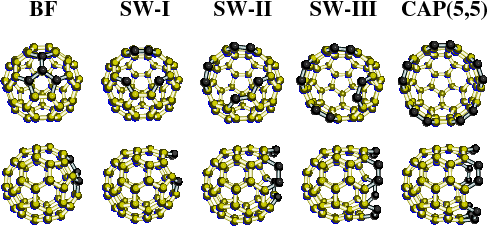
\includegraphics[width=12.5cm]{sample-fig1}}
    \caption{ Ball-and-stick models of meta-stable isomers in
        cage opening process from a C$_{60}$ buckminsterfullerene
        to a (5,5) capsule. We name them BF and CAP(5,5).
        Depending on the number of the Stone-Wales (SW) transformation,
        we call the intermediate isomers with SW-I, SW-II, and SW-III.
        Highlighted atoms are undercoordinated except BF.
    } \label{mag-fig1}
\end{figure}


In conclusion, we find metalstable C$_{60}$ isomers with open cage structure,
which show magnetic instability including favorable ferromagnetic spin configurations.
This could be a possible mechanism for recently reported room temperature ferromagnetism
in polymerized C$_{60}$ solids.


\section{C/BN heterostructured nanotubes}

In conclusion, we used local spin density functional calculations
to study the occurrence of magnetism in quasi one-dimensional
heterostructured C/BN nanotubes free of metallic impurities. At
the zigzag boundary connecting carbon and boron nitride segments
of tubes, we found atomic-like states that acquire magnetization
when partly filled. Whereas individual C/BN heterojunctions can
be used to spin polarize electrons during transport, periodic
arrangements of heterojunctions in doped systems can lead to the
formation of a one-dimensional itinerant ferromagnetic state.


\chapter{Conclusion}

We discuss potentiality of metal-free ferromagnetism
in pure carbon systems and their hybrids.
We present possible C$_{60}$ isomers for occurrence of magnetic
instability.
Partly open cages with zigzag edges may play a crucial role in
the pure carbon magnets.
We also propose occurrence of one-dimensional magnetism in carbon and
BN heterostructured nanotubes.
Due to the doubly degenerated states at the borders between
carbon and BN nanotube segments, we find that Hund's rule-type
occupation occurs when we dope the systems.
When the adjacent border states overlap with each other,
our calculations show that magnetic ordering is favorable.

%%
%% 참고문헌 시작
%% Refences
%%
\begin{thebibliography}{00}

\bibitem{Iijima91} S. Iijima,
         Nature (London) {\bf 354}, 56 (1991).
         %Helical microtubules of graphitic carbon.

\bibitem{Dresselhaus96} M. S. Dresselhaus, G. Dresselhaus, and P. C. Eklund.
         {\em Science of Fullerenes and Carbon Nanotubes} (Academic, San Diego, 1996).

\bibitem{Saito98} R. Saito, G. Dresselhaus, and M. S. Dresselhaus,
         {\em Physical Properties of Carbon Nanotubes}
         (Imperial College Press, London, 1998).

\bibitem{Makarova01} T.L. Makarova, B. Sundqvist,
         R. H\"ohne, P. Esquinazi, Y. Kopelevich, P. Scharff,
         V.A. Davydov, L.S. Kashevarova, and A.V. Rakhmanina,
         Nature (London) {\bf 413}, 716 (2001).

\bibitem{Palacio01} F. Palacio, Nature (London) {\bf 413}, 690 (2001),
         and references therein.

\bibitem{SW} A.J. Stone and D.J. Wales,
         Chem. Phys. Lett {\bf 128}, 501 (1986).

\end{thebibliography}

%%
%% 한글요약문 시작 (Korean summary)
%%
%% Note. 영문논문일 경우에만 필요하니 한글논문의 경우에는 작성하지 마십시오.
%%
\begin{summary}

    지난 10여 년간 탄소 나노튜브는 자체의 독특한 전기적, 기계적 성질로
    인하여 다가오는 나노기술 분야의 이상적인 기초물질중의 하나로 떠오르고
    있다. 흑연을 감는 세세한 방법에 따라 전기적 특성이 금속성에서 1eV의
    띠간격을 가지는 반도체 특성까지 다양한 분포로 존재한다.
    본 학위논문에서는 탄소 나노튜브의 여러 물리적 성질에 대해 고찰하는데,
    기본적으로 제일원리 밀도함수 이론과 밀접결합근사 모형을 사용하여 전기적
    특성과 그 제어 방법, 자기적 특성, 그리고 수송특성 등을 다루고자 한다.

\end{summary}

%%
%% 감사의 글 시작
%% Acknowledgement
%%
% @command acknowledgement 감사의글
% @options [default: 클래스 옵션 korean|english ]
% - korean : 한글타이틀 | english : 영문타이틀

\acknowledgement[korean]

    이 논문을 완성하기까지 주위의 모든 분들로부터 수많은 도움을 받았습니다.

    끝으로 오늘의 제가 있을 수 있도록 사랑으로 키워 주신
    어머니와 또한 가족들에게 감사드립니다.
    저의 이 작은 결실이 그분들께 조금이나마 보답이 되기를 바랍니다.

%%
%% 이력서 시작
%% Curriculum Vitae
%%
% @command curriculumvitae 이력서
% @options [default: 클래스 옵션 korean|english ]
% - korean : 한글이력서 | english : 영문이력서
\curriculumvitae[korean]

    % @environment personaldata 개인정보
    % @command     name         이름
    %              dateofbirth  생년월일
    %              birthplace   출생지
    %              domicile     본적지
    %              address      주소지
    %              email        E-mail 주소
    % - 위 6개의 기본 필드 중에 이력서에 적고 싶은 정보를 입력
    % input data only you want
    \begin{personaldata}
        \name       {김 용 현}
        \dateofbirth{1972}{3}{25}
        \birthplace {대전 대덕구 평촌동 ...}
        \domicile   {대전 유성구 신성동 ...}
        \address    {대전 유성구 구성동 ...}
        \email      {yonghyunkim@test.kaist.ac.kr}
    \end{personaldata}

    % @environment education 학력
    % @options [default: (none)] - 수학기간을 입력
    \begin{education}
        \item[1988. 3.\ --\ 1990. 2.] 대전과학고등학교 (2년 수료)
        \item[1990. 3.\ --\ 1997. 2.] 한국과학기술원 물리학과 (B.S.)
        \item[1997. 3.\ --\ 1999. 2.] 한국과학기술원 물리학과 (M.S.)
    \end{education}

    % @environment career 경력
    % @options [default: (none)] - 해당기간을 입력
    \begin{career}
        \item[1997. 3.\ --\ 1999. 2.] 한국과학기술원 물리학과 일반조교
        \item[2001. 7.\ --\ 2002. 1.] 한국과학기술정보연구원 슈퍼컴퓨팅센터 위촉연구원
        \item[2002. 8.\ --\ 2002. 12.] 한국표준과학연구원 연구생
    \end{career}

    % @environment activity 학회활동
    % @options [default: (none)] - 활동내용을 입력
    \begin{activity}
        \item J. Choi, \textbf{Yong-Hyun Kim}, K.J. Chang, and D. Tomanek,
             \textit{Occurrence of itinerant ferromagnetism in C/BN superlattice
             nanotubes}, 5th Asian Workshop on First-Principles Electronic
             Structure Calculations, Seoul (Korea), October., 2002.
    \end{activity}

    % @environment publication 연구업적
    % @options [default: (none)] - 출판내용을 입력
    \begin{publication}
        \item \textbf{Yong-Hyun Kim}, J. Choi, K.J. Chang, and D. Tomanek,
             \textit{Magnetic instability in partly opened C$_{60}$ isomers},
             in preparation.
    \end{publication}

%% 본문 끝
\end{document}
